% =========================================================================
% Secao 6C - Iteracao das taxas e conclusao
% =========================================================================

\section{Iteração das taxas de transição e taxa de conclusão observada}
\label{sec:iteracao}

Esta seção apresenta um exercício de consistência entre as taxas
de transição reportadas pelo INEP e pela PNADC e a taxa de
conclusão do ensino fundamental e do ensino médio observada
diretamente nos dados da PNADC via a variável \texttt{VD3004},
que reporta o nível de instrução mais elevado alcançado pelo
respondente. A pergunta é simples e tem resposta de grande
utilidade prática. Se aplicarmos iterativamente as taxas anuais
do INEP e da PNADC a uma coorte sintética que inicia o primeiro
ano do EF, qual taxa de conclusão do EF e do EM estaria
projetada? Essa projeção é consistente com a conclusão observada
entre jovens adultos na PNADC?

A construção do exercício é a seguinte. Tomamos uma coorte de
cem crianças entrando no primeiro ano do EF no ano $y_0 = 2005$.
Em cada ano subsequente, aplicamos as taxas médias do INEP do
período 2014--2019, separadamente para cada série do EF e do
EM, e contabilizamos a fração da coorte promovida, retida,
evadida e migrada para EJA. Iteramos por vinte anos, tempo
suficiente para que mesmo coortes com defasagem severa cheguem
ao terceiro ano do EM. Ao final, contamos como concluintes do
EF as crianças promovidas do nono ano do EF, e como concluintes
do EM as promovidas do terceiro ano do EM, em qualquer ano da
janela simulada. O mesmo exercício é repetido aplicando as
taxas médias da PNADC v5 do período 2017--2019, na versão
calibrada da Tabela~\ref{tab:t1_brasil}.

Em paralelo, computamos a conclusão observada diretamente na
PNADC. Para cada ano-calendário entre 2012 e 2024, identificamos
o conjunto de jovens adultos com idade entre dezenove e vinte e
quatro anos, faixa em que a maioria dos que iriam concluir o EF
e o EM já o teriam feito. Em seguida, calculamos a fração com
\texttt{VD3004} igual ou superior a três (EF completo) e a
fração com \texttt{VD3004} igual ou superior a cinco (EM
completo), ponderada pelo peso amostral. A
Tabela~\ref{tab:t7_completion} sintetiza os três indicadores
para o ano de 2019.

% C18b v5 iterative completion
\begin{table}[htbp]\centering
\caption{Taxa de conclus\~ao do EF e do EM: simula\c{c}\~ao de coorte (INEP), simula\c{c}\~ao de coorte (PNADC v5) e taxa observada (PNADC, jovens 19--24).}
\label{tab:t7_completion}
\begin{threeparttable}\small
\begin{tabular}{lrr}\toprule
Fonte & Concl.\ EF (\%) & Concl.\ EM (\%) \\\midrule
INEP (projetada) & 68.7 & 46.3 \\
PNADC v5 (projetada) & 68.8 & 47.0 \\
PNADC (observada 2019, 19-24) & 88.3 & 68.2 \\
\bottomrule\end{tabular}
\begin{tablenotes}\footnotesize
\item \textit{Fontes:} INEP Indicadores de Trajet\'oria (m\'edia 2014--2019) e PNADC v5 (m\'edia 2017--2019, com corre\c{c}\~ao V3014).
\item \textit{Notas:} Simula\c{c}\~ao iterativa de 100 crian\c{c}as entrando no 1\textsuperscript{o} EF, aplicando taxas por s\'erie ao longo de 20 anos. A taxa observada PNADC \'e o percentual de jovens de 19--24 anos em 2019 com \texttt{VD3004} indicando conclus\~ao do n\'ivel correspondente.
\end{tablenotes}\end{threeparttable}\end{table}


O resultado é instrutivo de duas formas. Em primeiro lugar, a
simulação iterativa com as taxas do INEP e a simulação com as
taxas da PNADC v5 produzem resultados praticamente idênticos.
INEP projeta conclusão do EF de 68,7\% e do EM de 46,3\%, ao
passo que PNADC v5 projeta 68,8\% e 47,0\%, respectivamente. A
proximidade entre as duas projeções é evidência forte de que a
calibração v5, com a correção \texttt{V3014} e a janela
$Q_2$--$Q_3$, alinha a metodologia operacional da PNADC com a
do INEP no que diz respeito ao fluxo anual médio. Em segundo
lugar, ambas as projeções ficam aproximadamente vinte pontos
percentuais abaixo da conclusão observada entre jovens adultos
de dezenove a vinte e quatro anos em 2019, que é de 88,3\% para
o EF e 68,2\% para o EM. A discrepância entre projeção e
observação é portanto sistemática e cobre tanto a fonte
administrativa (INEP) quanto a fonte domiciliar (PNADC).

A Figura~\ref{fig:completion_compare} mostra as séries temporais
correspondentes. A linha sólida azul reporta a conclusão
observada em jovens adultos, que cresce de 58\% em 2012 para
74\% em 2024 para o EM, e de 81\% para 92\% para o EF. As
linhas tracejadas horizontais correspondem aos níveis projetados
pela iteração das taxas do INEP e da PNADC, praticamente
sobrepostas e ambas abaixo da trajetória observada.

\begin{figure}[htbp]
\centering
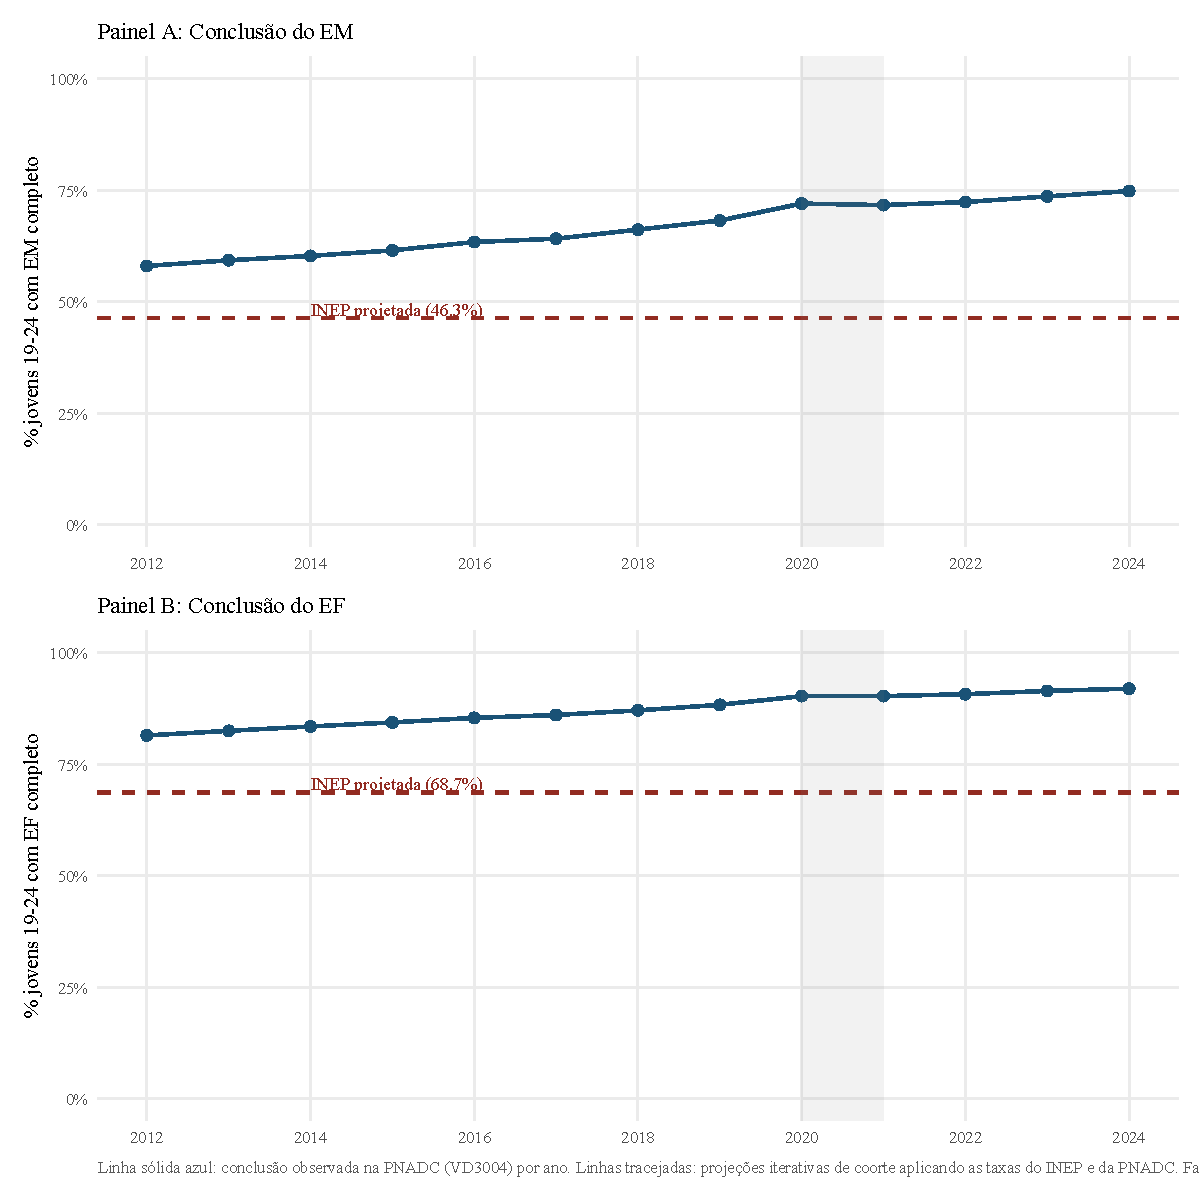
\includegraphics[width=0.95\textwidth]{../DataWork/5_Figures/output/F9_completion_comparison.pdf}
\caption{Taxa de conclusão do EM (Painel A) e do EF (Painel B):
projeção iterativa de coorte com taxas INEP e PNADC v5 versus
conclusão observada na PNADC.}
\label{fig:completion_compare}
\end{figure}

A interpretação metodológica desse exercício é a seguinte. As
taxas anuais de transição, tanto do INEP quanto da PNADC v5,
constituem em conjunto um \emph{limite inferior} sobre a taxa
de conclusão. Aplicadas iterativamente sob a hipótese de que
evasão é permanente e que repetentes são promovidos
eventualmente à mesma taxa anual, elas projetam uma conclusão
menor do que a observada em jovens adultos. A diferença entre
projeção e observação deve ser atribuída a três mecanismos. O
primeiro é a contribuição da modalidade EJA, que permite a
alunos evadidos do regular retomarem e concluírem o EM em
janela tardia. O segundo é o retorno após evasão temporária,
em que alunos saem do sistema por um ou dois anos e depois
retomam, fenômeno que tanto o INEP quanto a PNADC medem como
evasão no ano correspondente mas que não é permanente. O
terceiro é o conceito de evasão das duas fontes, que pode
incluir como evadidos alunos que apenas mudaram de modalidade,
de rede ou de UF, conforme discutido na Seção~\ref{sec:razoes}.

Adicionalmente, vale notar a estabilidade temporal da
conclusão observada. Entre 2012 e 2019, a conclusão do EM
entre jovens de dezenove a vinte e quatro anos cresceu de
58,0\% para 68,2\%, ganho de aproximadamente dez pontos
percentuais em sete anos. A partir de 2020, observa-se um
salto associado ao período COVID, provavelmente refletindo
políticas de aprovação automática e ajustes administrativos, e
o nível pós-pandemia em 2024 é de 74,8\%. Esse padrão é
compatível com a melhoria gradual do sistema educacional
brasileiro nas duas últimas décadas, ainda que com ritmo
modesto e com gargalo persistente no EM.

A conclusão substantiva é dupla. Primeiro, a convergência
entre INEP e PNADC v5 nas projeções iterativas valida a
calibração metodológica adotada nesta nota e confirma que as
duas fontes, após calibração, são equivalentes para
finalidades de medida de fluxo anual médio. Segundo, ambas as
fontes devem ser interpretadas como medidas de fluxo
\emph{instantâneo}, sensíveis a movimentos entre redes e a
interrupções temporárias, e não como medidas diretas de
trajetória cumulativa. Para finalidades de monitoramento de
políticas focalizadas, como o Pé-de-Meia, recomenda-se
reportar em paralelo dois indicadores complementares, isto é,
a taxa de fluxo anual e a taxa de conclusão observada em
jovens adultos, que juntos oferecem uma imagem mais completa
do desempenho do sistema educacional do que qualquer um deles
isoladamente.
